\documentclass[12pt,titlepage]{report}
\usepackage[a4paper, left = 2.5cm, right = 2.5cm, top = 1.5cm, bottom = 1.5cm, includeheadfoot]{geometry}
\usepackage[utf8]{inputenc}
\usepackage{graphicx}
\usepackage[english]{babel}
\usepackage[backend=biber, sorting=none, url=true, style=numeric]{biblatex}
\addbibresource{./references.bib}
\usepackage[hidelinks]{hyperref}
\usepackage[capitalize, noabbrev]{cleveref}
\usepackage{csquotes}

\usepackage{tocloft}
\tocloftpagestyle{empty}

\usepackage{titlesec}
\titleformat{\chapter}{\normalfont\huge\bfseries}{\thechapter .}{20pt}{\huge}
\titlespacing{\chapter}{0pt}{0pt}{1cm}

\usepackage{parskip}
\setlength{\parindent}{0pt}
\setlength{\parskip}{1em}
\renewcommand{\baselinestretch}{1.5}

\usepackage{caption}
\usepackage{subcaption}

\usepackage[capitalize, noabbrev]{cleveref}

\frenchspacing
\emergencystretch=1em

% Title Page
\title{\emph{slicevis} Python Package \\ \vspace{1cm} {Final Project for\\ \emph{Sustainable Computational Engineering} \\ RWTH Aachen University}}
\author{Nicholas Book \\ \href{mailto:nicholas.book@rwth-aachen.de}{nicholas.book@rwth-aachen.de}}
\date{14.08.2022}

\begin{document}

\maketitle
\tableofcontents
\clearpage
\setcounter{page}{1}
\chapter{Background}

Introduction?

What is this report about and how is it structured.

\section{Sustainable Computational Engineering}

Briefly summarize the principles and methods of sustainable (scientific) software development.

\section{Biomedical Imaging}

Give an overview of the field and of the imaging modalities. Name some applications of imaging (research and medical practice).

\section{Aim of Final Project}

What is the motivation for slicevis?
What were the concrete goals and desired features?
How is it useful?
Emphasize the focus on usability, maintainability (documentation), and reproducability.

The aim of my project is to develop a Python package that offers interactive visualization of slices of three-dimensional images. The package should support a wide range of file formats (e.g. Nifti, GFF, ...) and consolidate the datasets with associated metadata into an \enquote{Image} class. Furthermore, segmentations of the images...
\chapter{Package Structure}
This chapter details the structure of the \emph{slicevis} package repository which is publicly available on GitLab \cite{repo}.

Besides the Python source code for the package, located in the \texttt{slicevis} sub-directory, the repository contains a \texttt{README}, a license file (\texttt{LICENSE}), and build instructions for \texttt{pip}. Additionally, there is an directory for examples and one for documentation. 

The README is formatted using Markdown and it serves as a short description and usage guide for the package. 

Build instructions for \texttt{pip} are specified in the files \texttt{pyproject.toml}, \texttt{setup.cfg}, and \texttt{setup.py} according to the Python Packaging User Guide \cite{pypa}. In \texttt{pyproject.toml}, the build tool is configured to Setuptools. All necessary package metadata and dependencies are specified in \texttt{setup.cfg}. The dependencies are \texttt{numpy}, \texttt{pygff}, \texttt{nibabel}, \texttt{matplotlib}, \texttt{plotly}, \texttt{ipywidgets}, \texttt{nbformat}, \texttt{wheel}, and \texttt{pandas}. A \texttt{setup.py} file is included for backwards-compatibility reasons, as described here \cite{legacy_config}.

The documentation directory includes the final presentation and this report as a PDF plus all required \LaTeX{} files to make further changes to the report.

In the examples directory, the user will find several datasets and a Jupyter notebook that demonstrates how to use the package. For the datasets,  a CT scan of a mouse, including a multi-organ segmentation, a CT scan of a human upper body with labeled lung tumors, and a prediction of a neural network for the same lung scan was chosen. More details are given in the following chapter titled \emph{Use-Cases}. A special license file \texttt{LICENSE.txt} is also included which details the origins and copyright notices for all examples.

\emph{slicevis} is licensed under the MIT License, which permits free use, modification, and redistribution as long as credit is given \cite{mit}. 
\chapter{Implementation}
This chapter deals with the implementation details of the \emph{slicevis} Python package.

The interactive GUI relies on several other packages, namely jupyter, ipywidgets, and plotly.  

The widget.py modules defines the SliceWidget class which creates the GUI and handles all user interaction. A three-dimensional Numpy Ndarray is passed to the class instance constructor. There is also an optional debug mode which enables an Output widget [] and layout borders for developers. The init method adds all buttons, creates layouts, and connects function callbacks. Each widget has at least one callback associated to it.

\begin{figure}[h]
	\centering
	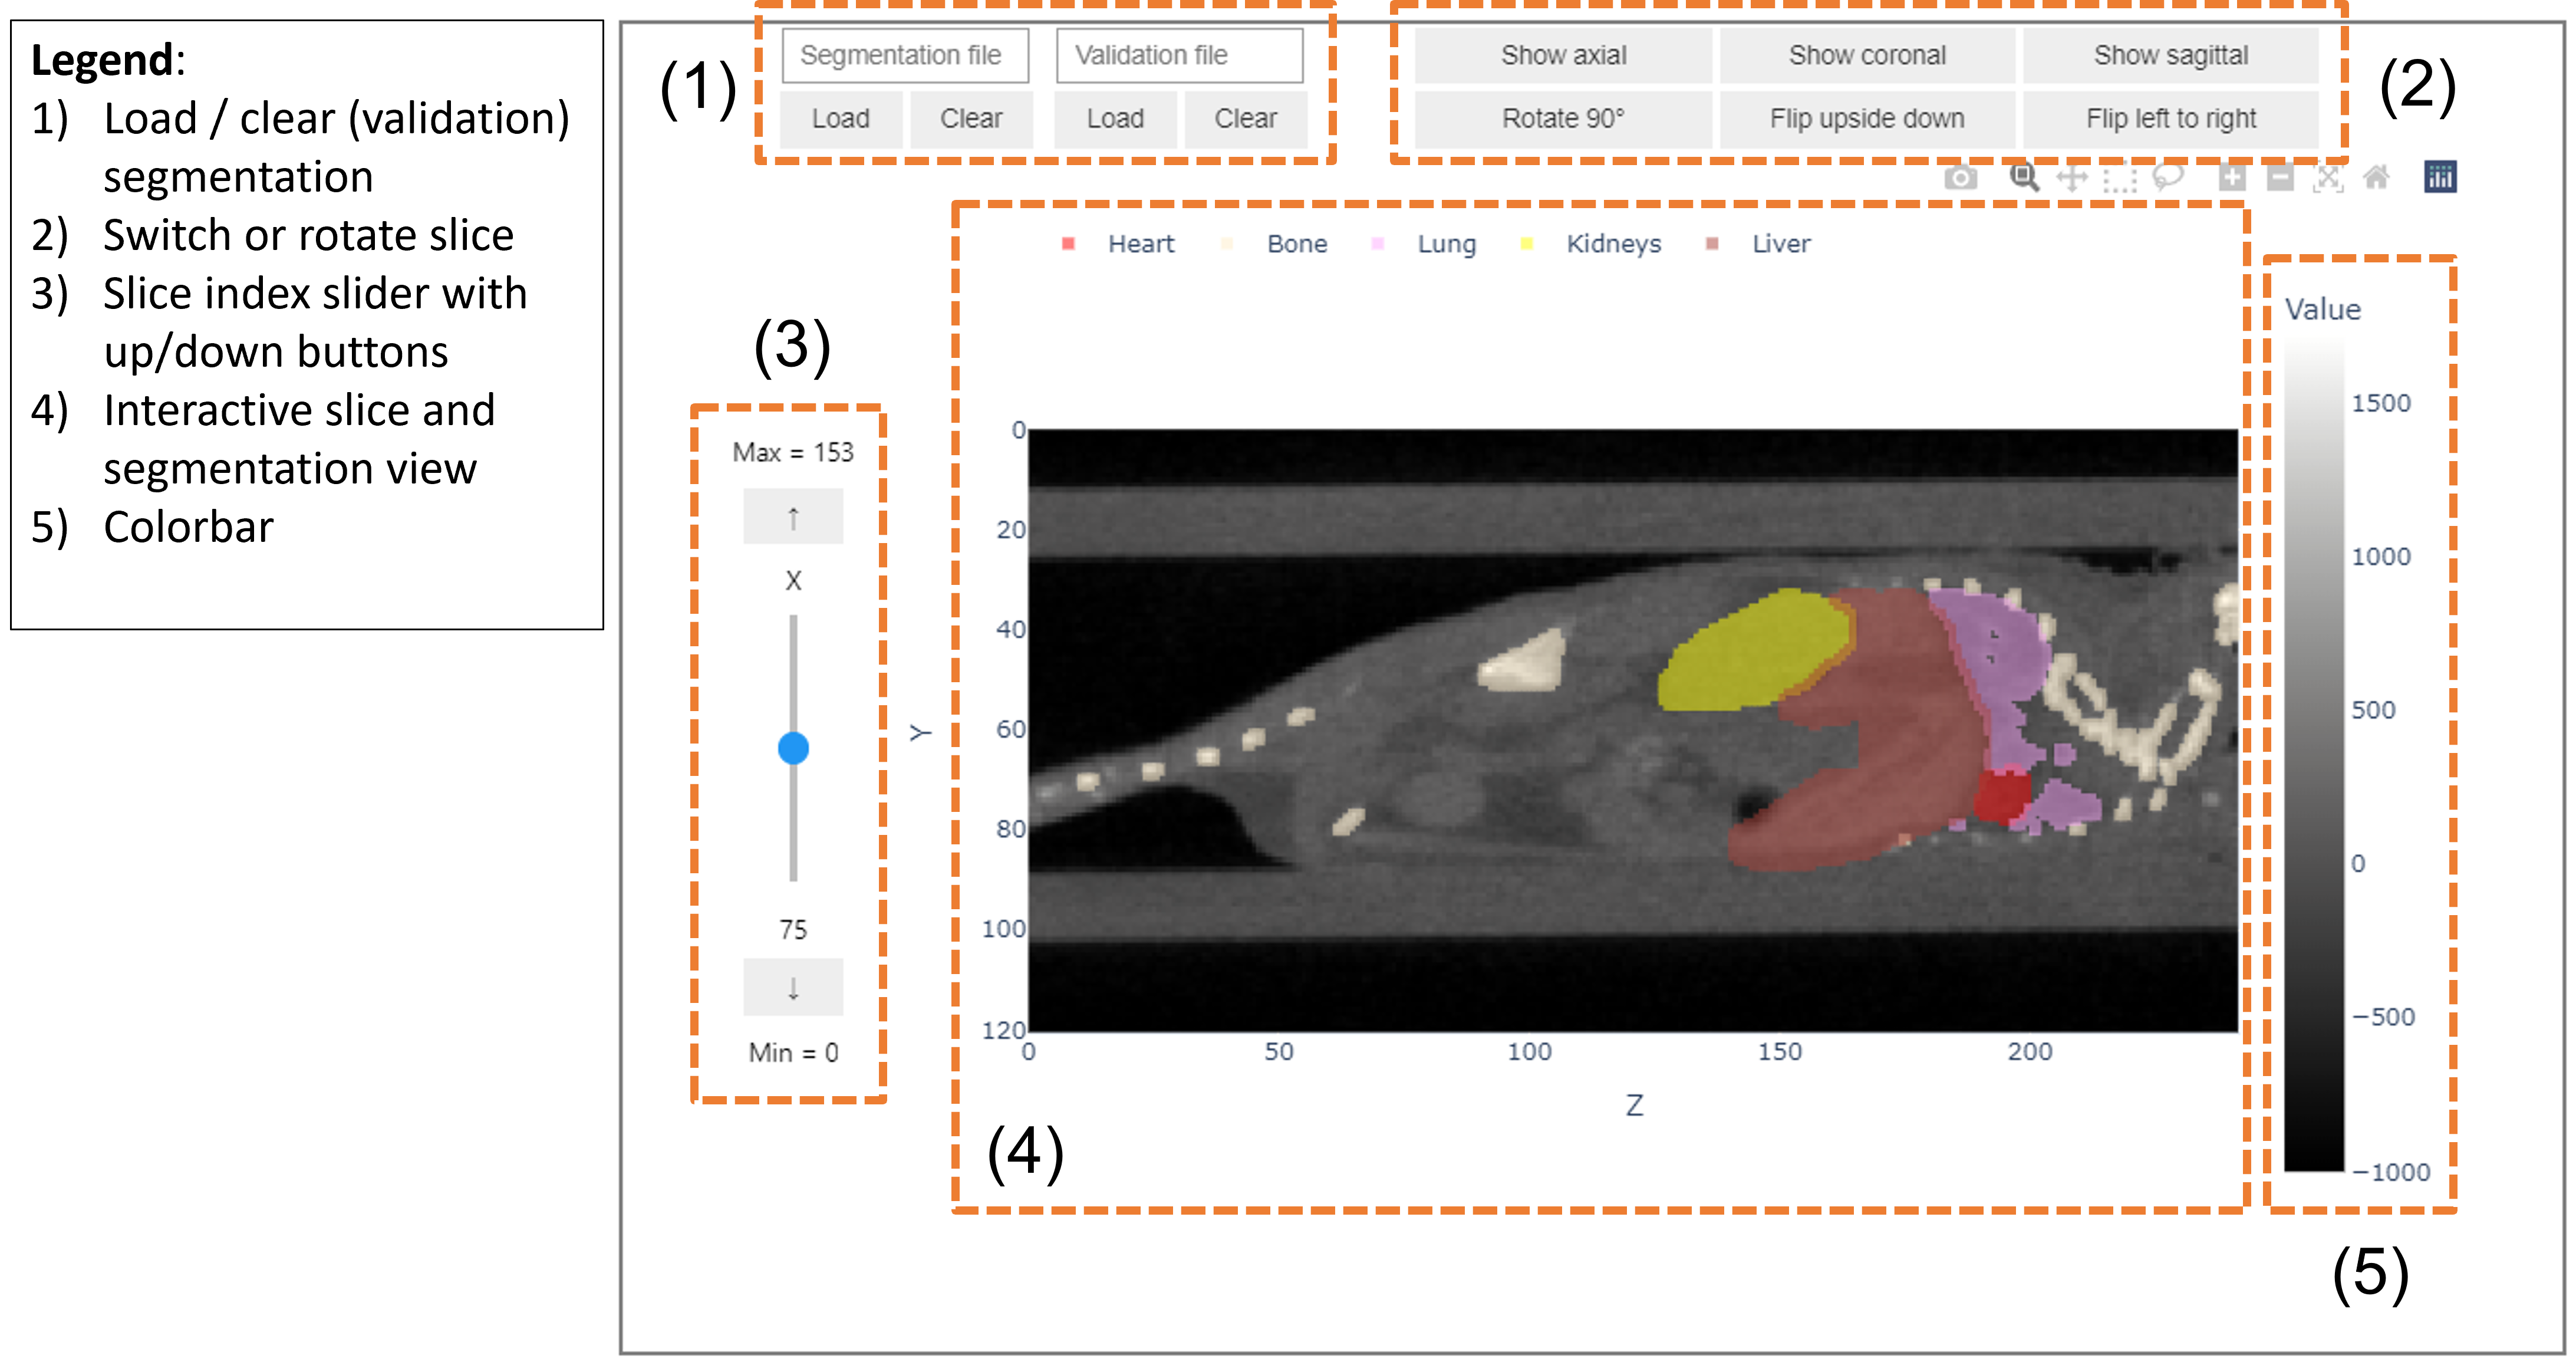
\includegraphics[width=.9\linewidth]{figures/GUI.png}
	\caption{The SliceWidget GUI, annotated.}
\end{figure}

Internally, the \_update2D method is the most important function as it responsible for setting the 2D image to the correct slice each time the user interacts with the widget. \_update2D also paints the (up to) two segmentations as scatter plots on top of the image. As this method is called multiple times per second for smooth slicing, it must be reasonably efficient in its implementation. Updating the 2D image is as simple as indexing into the (possibly rotated) 3D image in the current axis where the index is given as input to the callback. What is more tricky is painting the segmentations with their class names and colors on top. To find the pixels with coordinates $(x_i , y_i)$ of the class with index $j$ in the current slice, the Numpy method \emph{nonzero(condition)} is used. As \emph{condition}, one can ask where \emph{self.seg2D} $== j$. With the list of coordinate pairs, the class name, and its color, it is then possible to create a Plotly Scatter object and append it to the trace list. This is repeated for each segmentation class. In the end, a \emph{batch\_update()} is called on the widget where the 2D image is swapped out and the trace list is added on top. By batching the updates to the widget the render engine performs them all at once and flickering or delays are minimized. 

\begin{figure}[h]
	\centering
	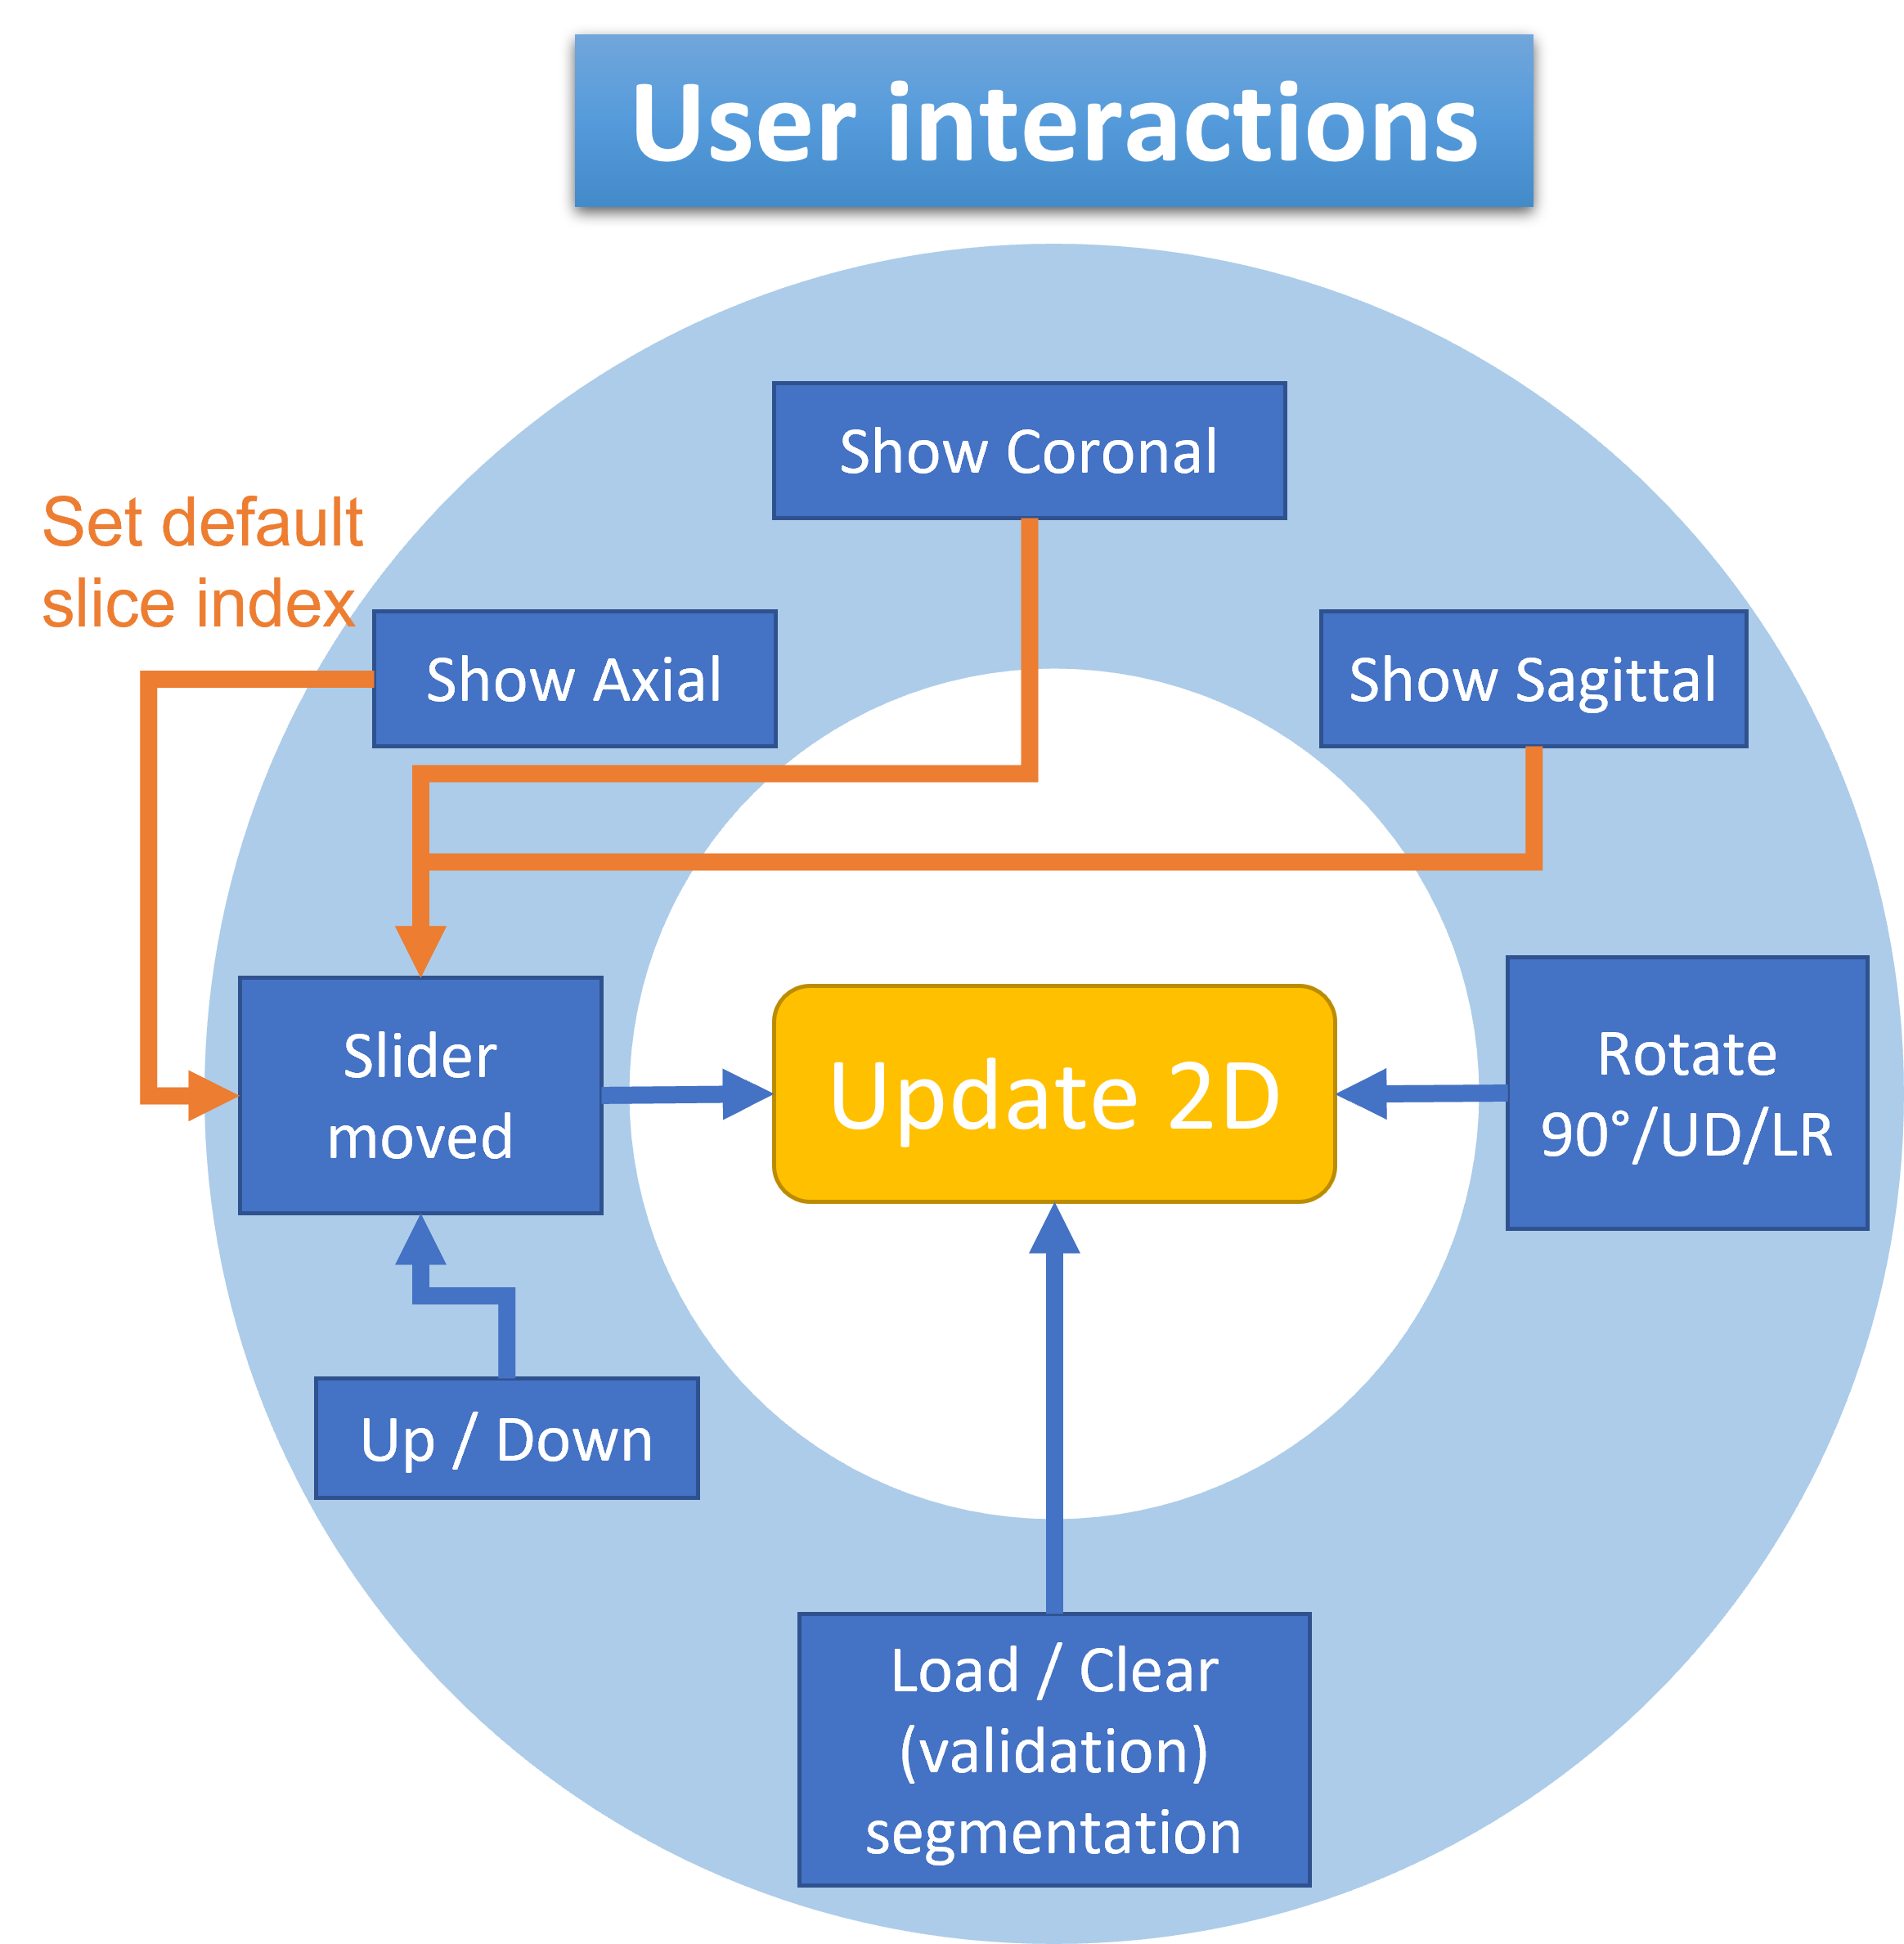
\includegraphics[height=.5\linewidth]{figures/call_graph.png}
	\caption{Call graph for interactive GUI update.}
\end{figure}

For more details, please refer to the documentation in the code.

DICE score computation:

\begin{equation}
	DICE(X, Y) =\frac{2|X \cap Y|}{|X|+|Y|}
\end{equation}
\chapter{Use Cases}

What can slicevis be used for? Example data is repo. Refer to license. 

\section{Whole-Body Murine CT Scans}

225 whole-body CT scans of lab mice. Two different resolutions.

Manual segmentations of all mayor organs included. By two trained experts.

GFF metadata includes name and color of each class. 

Screenshots of representative slices.

\section{The Cancer Imaging Archive}

95 CT scans of human upper bodies.

Republished as part of the Medical Segmentation Decathlon.

Very high resolution.

Labels of lung nodules included. Segmented by trained radiologist. 

Perfect for the training of CNNs.

\section{nnU-Net Prediction Validation}

Winning model of Decathlon challenge. Accuracy of 69\% for lung task.

Pre-trained model weights available for download. Network can be installed under Linux.

Prediction on one of the training cases is included in the repo. The aim is to validate the prediction using the DICE score.

Explain the DICE score. 

Automatically computed once a validation segmentation is loaded.

Screenshot of axial slice.
\printbibliography

\end{document}          
